\section{Background}
\label{sec:background}

Before we discuss FlowQoS's overall design we would like to introduce the concept of traffic policing and traffic shaping. While both techniques can be used for effectively limiting the rate at which traffic is forwarded through a link, these fundamentally differ in the way they handle the network packets.

Traffic policing is usually implemented using token-based approach where based on the set rate limit, a fixed number of tokens are allocated to an interface at the end of each token refresh period. As packets of corresponding sizes are forwarded the token count is reduced until no more tokens can be removed. This ensures that the interface does not send traffic more than the stipulated rate. However, if there are still packets left with the interface that could not be sent, the policer simply drops those packets. Also due to token based nature of policer, packet bursts get forwarded by the interface. The OpenvSwitch (OVS) ~\cite{ovs} implements rate limiting using traffic policing that is used by the FlowQoS's original architecture.

Traffic shaping, on the other hand, is implemented using a leaky-bucket approach (one variant of this is equivalent to a token-based approach) which in fact calculate an equivalent rate metric based on system architecture timer resolution and forwards traffic continuously strictly conforming to this rate. Any burst pf packets (packets at higher rate) are buffered in a short internal queue and delayed until the shaper acheives the desired transmission rate. Only when the queue becomes full, the residual packets are dropped. Due to this queuing, packets are expected slightly higher latencies than normal. The Hierarchical Token Bucket (HTB)~\cite{htb_manual} queuing discipline provided by the Linux's traffic control suite implements traffic shaping that follows a similar approach to forward traffic.

\begin{figure}[t]
\centering
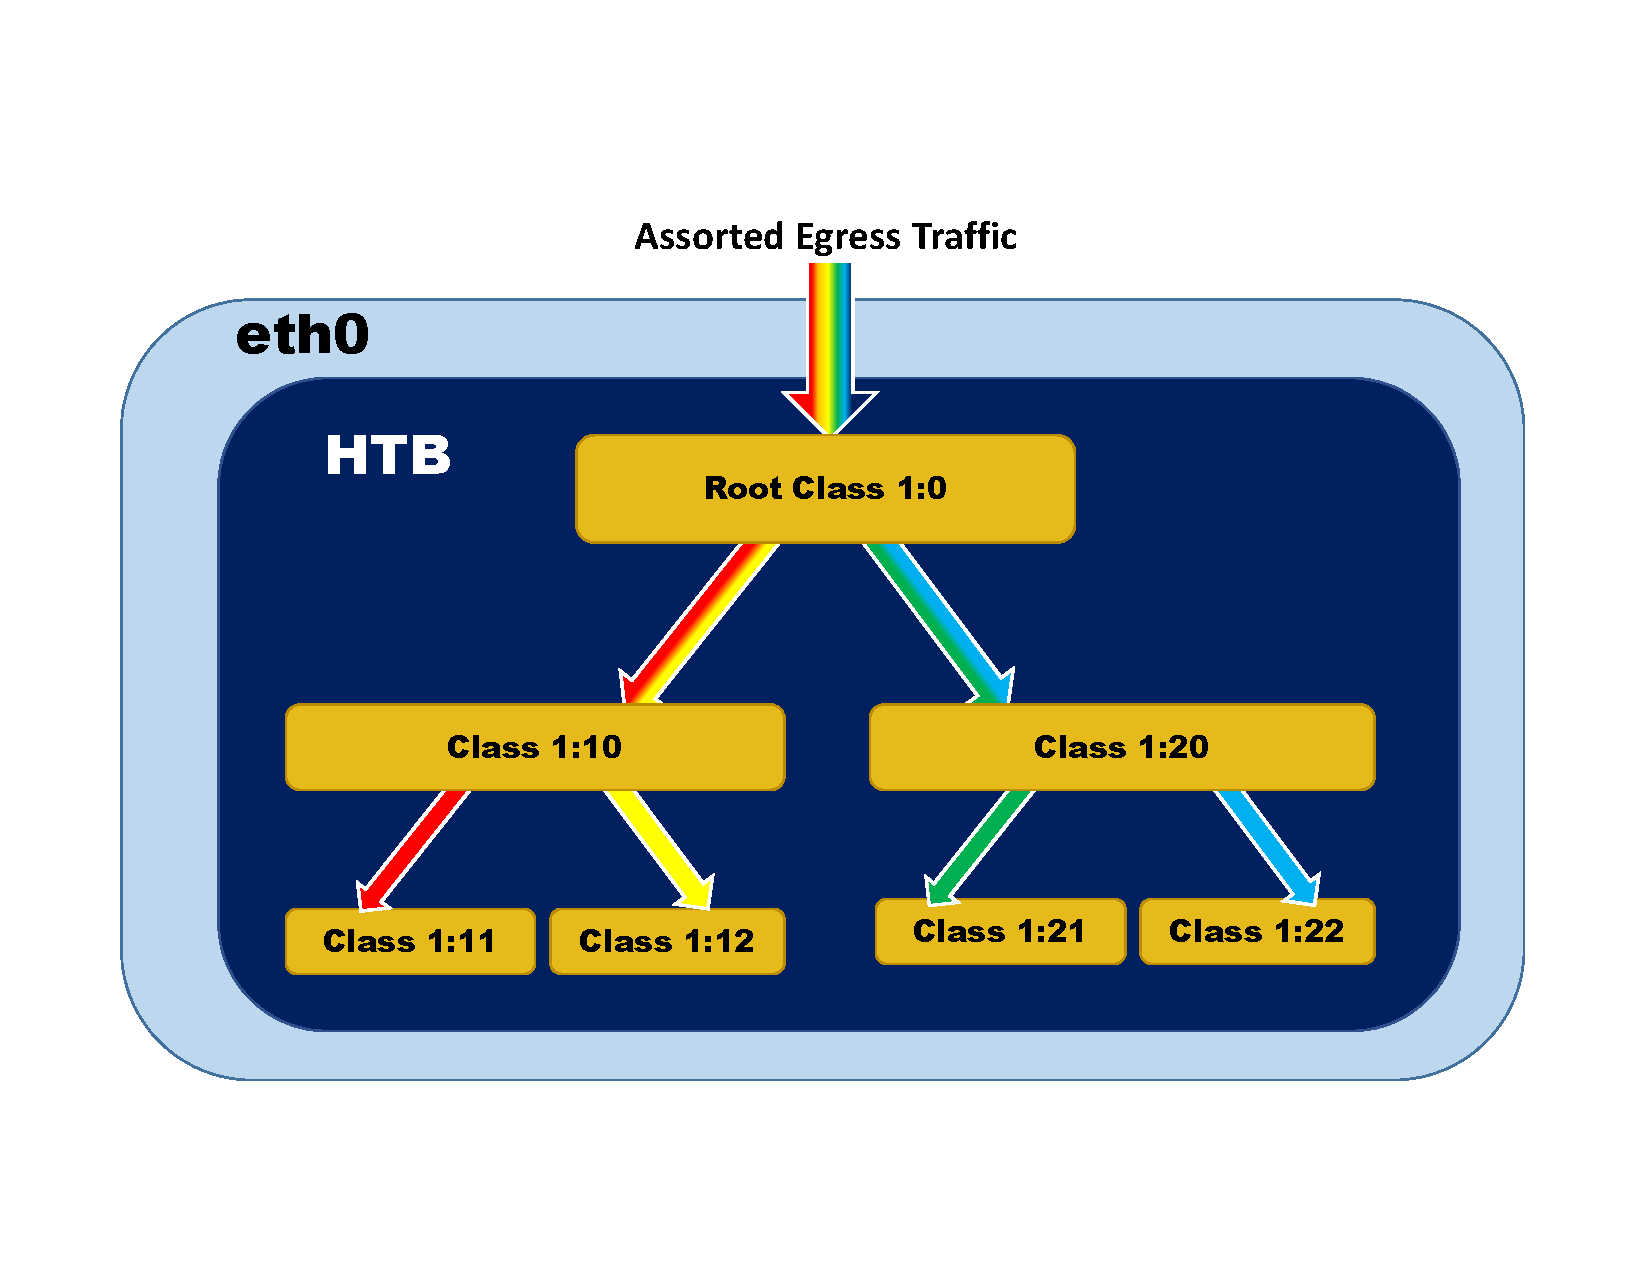
\includegraphics[width=0.9\linewidth]{LTC}
\caption{HTB Hierachical Class Structure Illustration.}
\label{fig:htb}
\end{figure}

Moreover, HTB is classful queuing discipline that allows adding multiple traffic filter (classes) under the root filter (class), which can further have sub-filters (sub-classes) forming a traffic classification tree. Each of the intermediate and leaf classes can have individual rate limits and therefore traffic shapers associated with them. In addition, they also have an associated priority that is respected by HTB while sharing unutilized bandwidth among multiple sibling classes. ~\fref{fig:htb} illustrates such a heirarchical structure described above and shows how egress traffic is partitioned into multiple classes.\\

%OVS and HTB both helps you to control a given link's outbound bandwidth. HTB is a quick, intuitive qdisc which is meant to be more understandable. It can send different kind of traffic on different links. To do this, we have to decide which link to use when a given packet is going to be sent.

%HTB can ensure that a service is provided with at least the minimum it requested by setting the rate on that class. If a class uses less than the rate it requested, the remaining bandwidth is being used by the other classes who needs more bandwidth. This is called borrowed bandwidth, and prioritizing decide who gets more bandwidth. 

%HTB decides how the bandwidth is being shared by comparing priorities. As we saw in OVS, only the rates are being considered. However, this could give bad utilization if a link uses less bandwidth than it initially is assigned to. 

%In HTB on the other hand, we use the borrowed bandwidth to exploit the unused bandwidth. Therefore, we are also able to assign the maximum bandwidth a class need. We do this by setting the ceiling-value for a class. The priorities of the classes and filters decides which class/qdisc get the available extra bandwidth.

%In HTB we use filters to classify the traffic when it enters a classful qdisc. To decide which class the packets should go to, we consult the filters. The filters attached to the classful qdisc return a decision to the qdisc. The qdisc then uses the decision to decide which class it should send the packet to.
%needs to be redone
%Prioritization of traffic has two crucial elements. First, it needs to tell how the excess bandwidth are distributed amongst siblings as mentioned above. HTB assigns excess bandwidth to the highest priority classes first. However, this allocation must consider the ceiling and rate rules which should always be followed. Second, when you prioritize one class to get less delay, the other classes will always have worse delay because of this. Therefore, when you prioritize packets, it's important to both consider the rate you give the class you prioritize, so you do not kill the other links.




%On figure \fref{figure:htb}, you can see a typical HTB-structure. Each class can have subclasses and filters. Here root class 1:0 is parent to class 1:10 and 1:20. The subclasses should have the same rate combined as their parent, and their ceiling should not go above their parents rate. 


